
\begin{tabular}{m{3cm}m{3cm}m{6cm} } 
	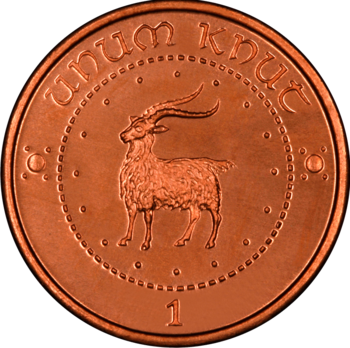
\includegraphics[width=3cm]{../Pictures/Gameplay/Items/Consumables/Currency/Knut_coin_picture.png} & \textbf{Knut} & A Knut, made out of bronze, is the least valued coin in British wizarding currency. There are 29 Knuts in one silver Sickle, and there are 493 Knuts in one golden Galleon. \\ 
	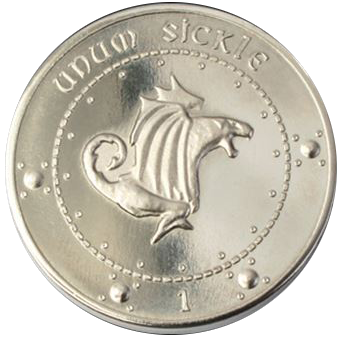
\includegraphics[width=3cm]{../Pictures/Gameplay/Items/Consumables/Currency/Sickle_coin_picture.png} & \textbf{Sickle} & A Sickle, made out of silver, is equal to 29 Knuts, and 17 Sickles make up a Galleon. \\ 
	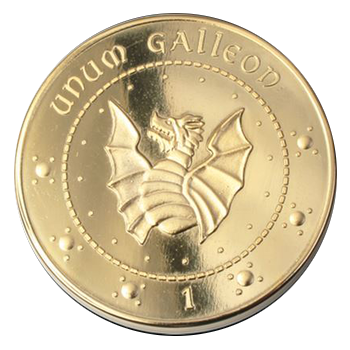
\includegraphics[width=3cm]{../Pictures/Gameplay/Items/Consumables/Currency/Galleon_coin_picture.png} & \textbf{Galleon} & A Galleon, made out of gold, is the most valued coin of the wizarding currency used in Britain. One Galleon is equal to 17 Sickles or 493 Knuts.  \\ 
	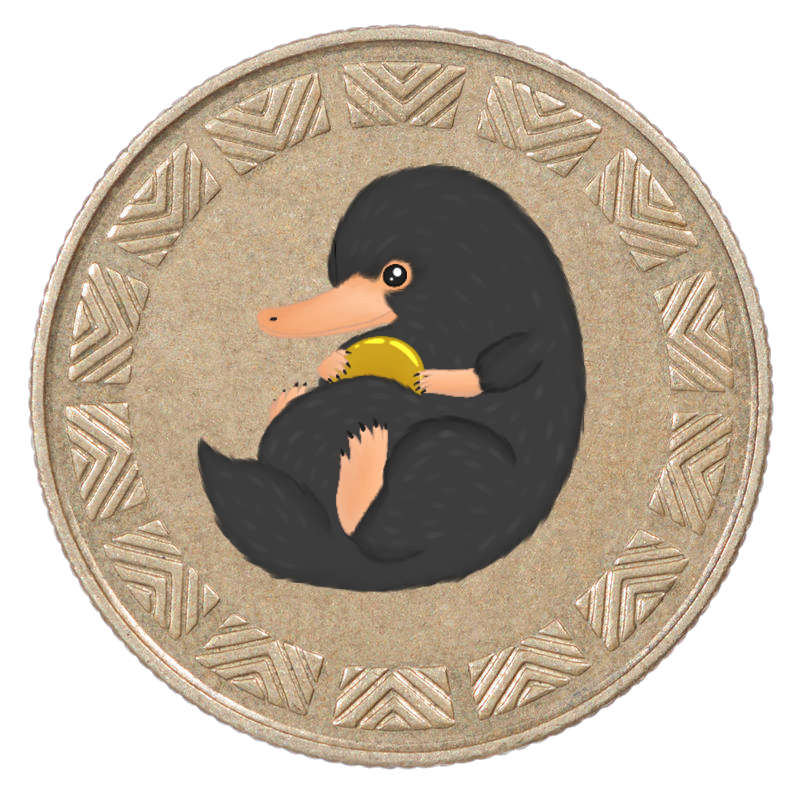
\includegraphics[width=3cm]{../Pictures/Gameplay/Items/Consumables/Currency/Niffler_coin_front_picture.png} & \textbf{Niffler Galleon} & Special currency, grants the blessing of the Niffler when used at their statues, acting as an effective checkpoint for the player. \\ 
\end{tabular}

\clearpage
